\chapter{Controller Design}\label{chap:Control}
The quadcopter system has been described with a mathematical model, for both the attitude and the translational behavior, \autoref{chap:Model}. This model is utilized when designing the different controllers. They are designed to fulfill the functional requirements stated in \autoref{ch:functionalRequirements}.

\autoref{fig:ControlHeadDiagram} shows the relation between the different controllers and models in the system.

% The attitude controller constitutes the inner loop, which is surrounded by the x and y translational controllers. An z controller, separated from attitude controller, handles the amount of thrust applied by the motors, by changing the required sum of their rotational speeds. 
%
\begin{figure}[H]
	\centering
	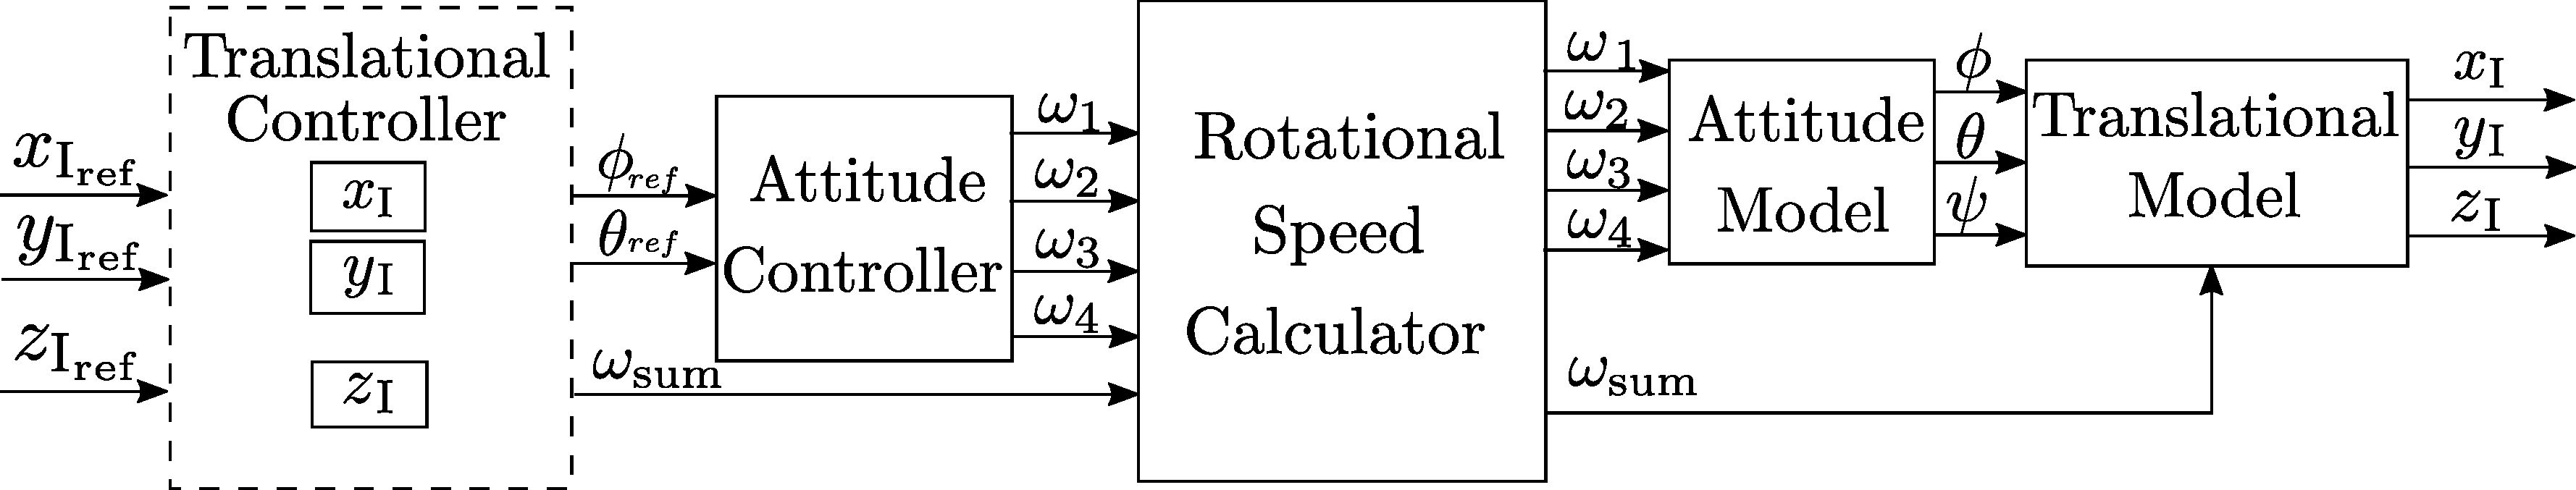
\includegraphics[width=1 \textwidth]{figures/generalcontroldiagram2}
	\caption{Block diagram of the overall control system.}
	\label{fig:ControlHeadDiagram}
\end{figure}
%
The translational controller, along $x_{\mathrm{I}}$, $y\mathrm{_I}$ and $z\mathrm{_I}$, are designed with classical control methods. These controllers receive $x_\mathrm{I_{ref}}$, $y_\mathrm{I_{ref}}$ and $z_\mathrm{I_{ref}}$ positions. The translational controllers for $x\mathrm{_I}$ and $y\mathrm{_I}$ constitutes an outer loop with the attitude controller as the inner loop. The $z\mathrm{_I}$ controller, separated from attitude controller, handles the amount of thrust applied by the motors, by changing the required sum of their rotational speeds. The attitude controller is designed using a state space approach. Note that the reference for yaw is not illustrated on the diagram, as it is set to zero so the quadcopter is able to move along $x_{\mathrm{I}}$ and $y\mathrm{_I}$ by changing $\theta$ and $\phi$, respectively.

The rotational speed calculator receives the speeds required by the attitude controller and the sum of speeds requested by the $z\mathrm{_I}$ controller. It combines the five inputs into the four motor rotational speeds applied to the system.

%takes into account the rotational speeds that the attitude controller needs in each motor and the sum that is needed to get the desired thrust in the $z_\mathrm{I}$ direction. Then, it combines both to give the final control action that is applied to the system.

This chapter starts by describing the attitude controller followed by the design of the translational controller. In the design process, simulations including the network effects and the model are depicted. The simulations also consider the sampling frequency, which is 28 Hz as described in \autoref{sec:ContDiscrete}. This ensures that the controllers yield a stable behavior and the references are tracked. 